\documentclass[journal,12pt,twocolumn]{IEEEtran}
\usepackage{setspace}
\usepackage{gensymb}
\singlespacing
\usepackage[cmex10]{amsmath}
\usepackage{amsthm}
\usepackage{mathrsfs}
\usepackage{txfonts}
\usepackage{stfloats}
\usepackage{bm} 
\usepackage{cite}
\usepackage{cases}
\usepackage{subfig}
\usepackage{tkz-euclide}
\usepackage{longtable}
\usepackage{multirow}
\usepackage{enumitem}
\usepackage{mathtools}
\usepackage{steinmetz}
\usepackage{tikz}
\usepackage{circuitikz}
\usepackage{verbatim}
\usepackage{tfrupee}
\usepackage[breaklinks=true]{hyperref}
\usepackage{graphicx}
\usepackage{tkz-euclide}
\usetikzlibrary{calc,math}
\usepackage{listings}
    \usepackage{color}                                            %%
    \usepackage{array}                                            %%
    \usepackage{longtable}                                        %%
    \usepackage{calc}                                             %%
    \usepackage{multirow}                                         %%
    \usepackage{hhline}                                           %%
    \usepackage{ifthen}                                           %%
    \usepackage{lscape}     
\usepackage{multicol}
\usepackage{chngcntr}
\DeclareMathOperator*{\Res}{Res}
\renewcommand\thesection{\arabic{section}}
\renewcommand\thesubsection{\thesection.\arabic{subsection}}
\renewcommand\thesubsubsection{\thesubsection.\arabic{subsubsection}}
\renewcommand\thesectiondis{\arabic{section}}
\renewcommand\thesubsectiondis{\thesectiondis.\arabic{subsection}}
\renewcommand\thesubsubsectiondis{\thesubsectiondis.\arabic{subsubsection}}
\hyphenation{op-tical net-works semi-conduc-tor}
\def\inputGnumericTable{}                                 %%
\lstset{
%language=C,
frame=single, 
breaklines=true,
columns=fullflexible
}
\begin{document}
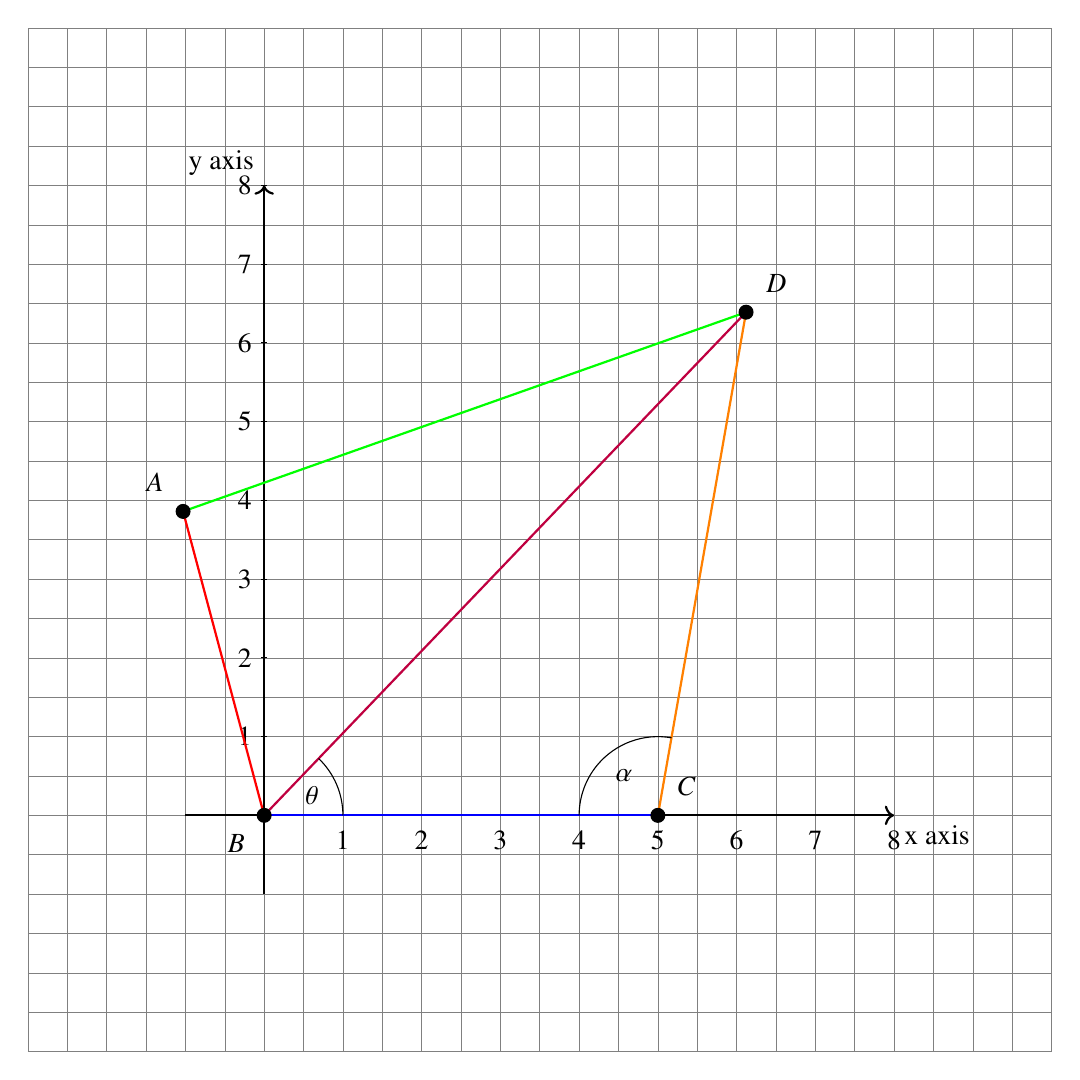
\begin{tikzpicture}
\centering
\draw[step=0.5cm,gray,very thin] (-3,-3) grid (10,10);
\draw[thick,->] (-1,0) -- (8,0) node[anchor=north west] {x axis};
\draw[thick,->] (0,-1) -- (0,8) node[anchor=south east] {y axis};
\foreach \x in {1,2,3,4,5,6,7,8}
   \draw (\x cm,-2pt) -- (\x cm,-2pt) node[anchor=north] {$\x$};
\foreach \y in {1,2,3,4,5,6, 7, 8}
    \draw (1pt,\y cm) -- (-1pt,\y cm) node[anchor=east] {$\y$};
\draw[blue,thick] 
(0,0)--(5,0);
\draw[orange,thick]
(5,0)--(6.12,6.39);
\draw[ green,thick]
(6.12,6.39)--(-1.03,3.86);
\draw[red,thick]
(-1.03,3.86)--(0,0);
\draw[purple,thick]
(0,0)--(6.12,6.39);
%Labeling points
\node (B) at (0, 0)[label=below left:$B$] {};
\node (C) at (5, 0)[label=above right:$C$] {};
\node (D) at (6.12,6.39)[label=above right:$D$] {};
\node (A) at (-1.03,3.86)[label=above left:$A$] {};
\filldraw (0,0) circle[radius=2.5pt,];
\filldraw (5,0) circle[radius=2.5pt];
\filldraw (6.12,6.39) circle[radius=2.5pt];
\filldraw (-1.03,3.86) circle[radius=2.5pt];
\tkzMarkAngle(C,B,D)
\tkzLabelAngle[pos = 0.6](C,B,D){$\theta$}
\tkzMarkAngle(D,C,B)
\tkzLabelAngle[pos = 0.6](D,C,B){$\alpha$}
\end{tikzpicture}
\end{document}